155. \begin{figure}[ht!]
\center{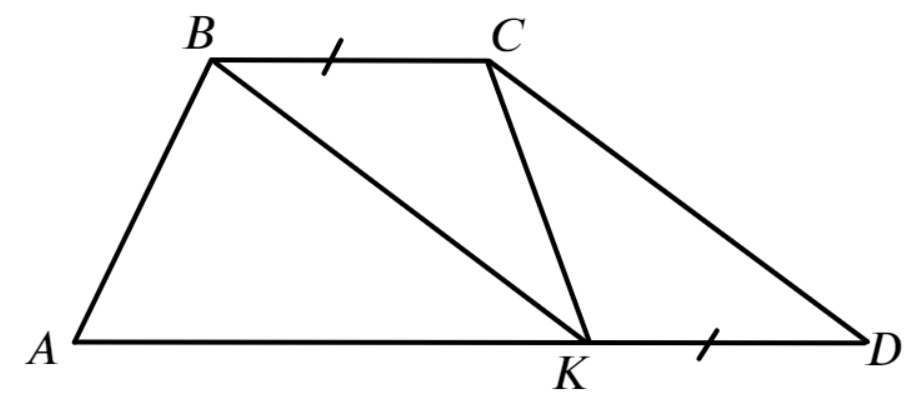
\includegraphics[scale=0.35]{g8-155.png}}
\end{figure}\\
Так как $(BC)\parallel (KD)$ и $(BK)\parallel(CD),$ четырёхугольник $BCDK$ является параллелограммом, а значит $KD=BC.$ Тогда $AK=AD-KD=\cfrac{12}{5}KD-KD=\cfrac{7}{5}KD,$ то есть $AK:KD=7:5.$ Диагональ $CK$ делит параллелограмм $BCDK$ на два равных треугольника, значит $S_{\Delta CKD}=S_{\delta BKC}=15.$ У треугольников $ABK$ и $CKD$ равны высоты, опущенные из точек $B$ и $C,$ значит $\cfrac{S_{\Delta ABK}}{S_{\Delta CKD}}=\cfrac{AK}{KD}=\cfrac{7}{5}$ и $S_{\Delta ABK}=\cfrac{7}{5}\cdot15=21.$ Таким образом, $S_{ABCD}=15+15+21=51.$
ewpage
oindent
